\chapter[Embasamento Teórico]{Embasamento Teórico}
\label{ch:cap2}
O \textit{Power Monitor} surgiu da necessidade da conscientização do gasto energético e da melhor compreensão da conta de luz. Baseado nesse conceito,
foram desenvolvido um \textit{software} que permitirá uma fácil comunicação com qualquer equipamento construido que tenha a finalizade de monitorar a energia elétrica.
O sistema traz uma forma mais fácil e próxima do consumidor final de se quantificar a energia elétrica consumido em um estabelecimento. No lugar do Quilowatt-hora, medida que é usada atualmente,
o \textit{software} propõe mensurar o gasto energético em reais (R\$), trazendo a realidade do consumo mensal para mais próximo de cada brasileiro.

Esse capítulo trará os conceitos essenciais para o entendimento do trabalho, descrevendo todas as tecnologias utilizadas no desenvolvimento 
do \textit{software} como do \textit{hardware}.

\section[\textit{Ferramentas e Linguagem}]{\textit{Ferramentas e Linguagem}}\label{ferramenta-linguagem}
No decorrer do desenvolvimento do \textit{software} fez-se uso de algumas tecnologias e linguagens de programação que serão descrita no decorrer
dessa seção.
\subsection[\textit{Node.js}]{\textit{Node.js}}\label{node}
Node.js é um interpretador do código JavaScript (\autoref{js}), com o foco do uso da linguagem do lado do cliente para servidores. Com um objetivo simples
que é ajudar desenvolvedores na criação de aplicações de alta escalabilidade, com códigos capazes de administrar e manipulazar várias conexões simultaneamente
em um único servidor. O \textit{Node.js} é baseado na \textit{runtime} V8 \textit{JavaScript Engine}. Foi desenvolvido por Ryan Danhl em 2009, e o seu desenvolvimento
é mantido pela fundação \textit{Node.js} e \textit{Linux Foundation}. 
\subsection[\textit{JavaScript}]{\textit{JavaScript}}\label{js}
JavaScript é uma linguagem de programação interpretada de alto nível, juntamente com HTML e CSS é uma das linguagens mais utilizadads no mundo \textit{web}.
Após o uso da linguagem as páginas \textit{web} começaram a ter uma maior interatividade com o usuário. A grande maioria dos \textit{browsers} tem um
mecanismo de compilação dedicado para o JavaScript. Por ser uma linguagem multi-paradigma o JavaScript suporta paradigmas funcionais, orientados a eventos 
e até mesmo paradigmas de orientação a objeto.
Inicialmente era usada apenas no lado do cliente em \textit{web browsers}, mas atualmente está presente em vários outros tipos de \textit{softwares} incluindo
servidores - como já foi discutido na \autoref{node} - \textit{databases} e até sistemas \textit{desktop} como os leitores de PDF, programas de música e recentemente
vem ganhando espaço no desenvolvimento de aplicativos para celular.

\subsection[\textit{WebSocket}]{\textit{WebSocket}}\label{websocket}
A ideia da tecnologia surgiu da problematica onde as comunicações entre servidor e aplicação era baseada na sobrecarga do HTTP, que não é indicado para aplicativos
com baixa latência. O WebSocket define uma API que estabelece a conexão de soquete entre aplicação e servidor, resumidamente é uma conexão, baseada no protocolo TCP, persistente
entre servidor e cliente onde ambas as partes podem enviar ou receber informações a qualquer momento. A forma como a conexão acontece é bem simples,
o cliente e o servidor antes de tudo devem negociar o \textit{handshake} - processo pelo qual os dois lados, geralmente cliente e servidor, passam para
reconhcimento de ambos os lados e concretizar a comunicação - de atualização do http e depois disso aplicar as regras assicronas do websocket, como mostra
a \autoref{fig:websocket-diagram}.

\begin{figure}[h!]
	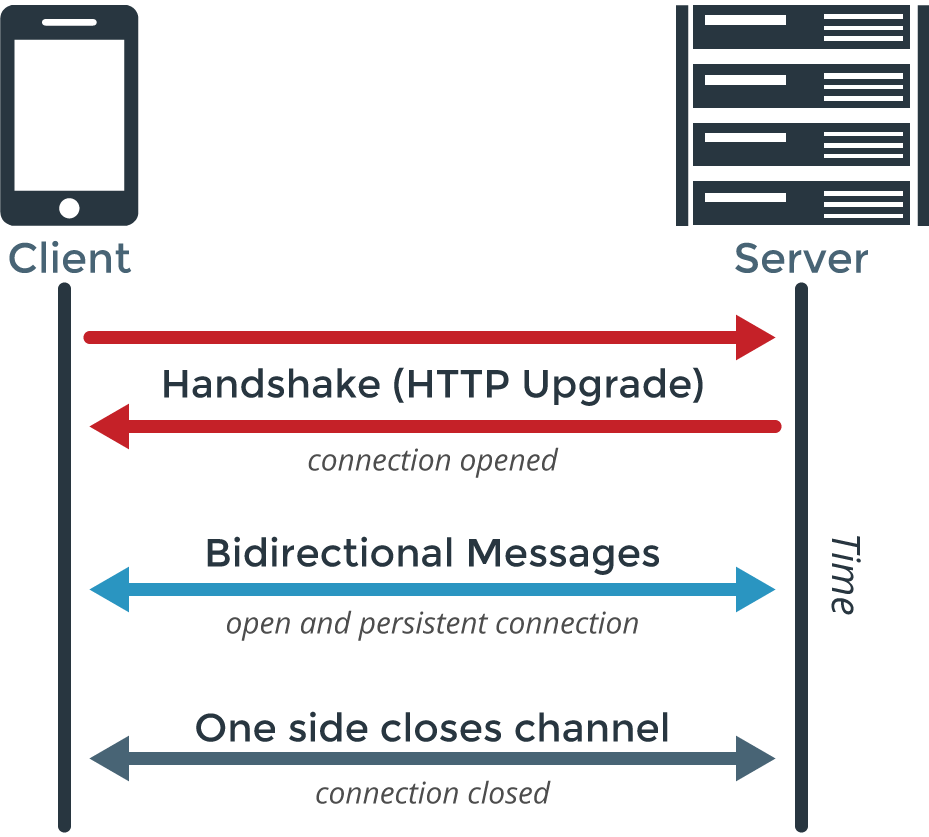
\includegraphics[width=0.6\textwidth, keepaspectratio=true]{websockets-diagram}
	\centering
	\caption[Diagrama de conexão via websocket]{Diagrama de conexão via websocket}
	\fonte{\url{https://www.pubnub.com/learn/glossary/what-is-websocket/}{}}
	\label{fig:websocket-diagram}
\end{figure}
\FloatBarrier


\subsection[\textit{SQL}]{\textit{SQL}}\label{sql}

\section[\textit{Componentes Físicos}]{\textit{Componentes Físicos}}\label{comp-fisico}
\subsection[\textit{ESP8266}]{\textit{ESP8266}}\label{esp}

%NodeJs
%javascript
%jquery
%websocket
%Sql
%Mysql
%esp8266
%componentes do circuito
